\documentclass[12pt,a4paper]{article}

\usepackage{graphicx}
\usepackage{geometry}
\usepackage{amsmath}
\usepackage{array}
\usepackage{fancyhdr}

\geometry{margin=1in}

\pagestyle{fancy}
\fancyhf{}
\rhead{PH 2019 - Question 26}
\lhead{Logic Gate Simplification}
\rfoot{\thepage}

\begin{document}

%================ LOGO ==================
\begin{center}
    
\includegraphics[width=3cm]{logo.jpeg}
\end{center}

\vspace{0.5cm}

%================ TITLE ==================
\begin{center}
    \Large\textbf{PH 2019 – Question 26 Analysis}
\end{center}

\vspace{0.5cm}

\noindent
\textbf{Name:} Jera Prakash \\
\textbf{ID:} COMETFWC038 \\
\textbf{Date:} 02-02-2026

\vspace{0.5cm}

%================ QUESTION ==================
\section*{Question}

Simplify the Boolean expression:

\[
F = (\overline{A} + \overline{B})[\overline{A(B + C)}] + A(\overline{B} + \overline{C})
\]

Identify the logic gate and verify using hardware implementation.

%================ ANALYSIS ==================
\section*{Step-by-Step Simplification}

Given:

\[
F = (\overline{A} + \overline{B})[\overline{A(B + C)}] + A(\overline{B} + \overline{C})
\]

Using DeMorgan's Law:

\[
\overline{A(B+C)} = \overline{A} + \overline{(B+C)}
\]

\[
= \overline{A} + \overline{B}\,\overline{C}
\]

Substituting:

\[
F = (\overline{A} + \overline{B})(\overline{A} + \overline{B}\overline{C}) + A(\overline{B} + \overline{C})
\]

Using identity:

\[
(X+Y)(X+Z) = X + YZ
\]

\[
F = \overline{A} + \overline{B}\overline{C} + A\overline{B} + A\overline{C}
\]

Simplifying:

\[
F = \overline{A} + \overline{B} + A\overline{C}
\]

Further simplification:

\[
F = \overline{A} + \overline{B} + \overline{C}
\]

Using DeMorgan's Law:

\[
F = \overline{A \cdot B \cdot C}
\]

\textbf{Final Simplified Expression:}

\[
\boxed{F = \overline{ABC}}
\]

%================ TRUTH TABLE ==================
\section*{Truth Table}

\begin{center}
\begin{tabular}{|c|c|c|c|}
\hline
A & B & C & F \\
\hline
0 & 0 & 0 & 1 \\
0 & 0 & 1 & 1 \\
0 & 1 & 0 & 1 \\
0 & 1 & 1 & 1 \\
1 & 0 & 0 & 1 \\
1 & 0 & 1 & 1 \\
1 & 1 & 0 & 1 \\
1 & 1 & 1 & 0 \\
\hline
\end{tabular}
\end{center}

%================ HARDWARE ==================
\section*{Hardware Implementation}

The simplified logic represents a 3-input NAND gate.

It is implemented using Raspberry Pi Pico 2 W and a 7-segment display.

\subsection*{Required Components}

\begin{itemize}
    \item Raspberry Pi Pico 2 W
    \item Breadboard
    \item 7-Segment Display
    \item 220$\Omega$ Resistor
    \item Jumper Wires
    \item USB Cable
\end{itemize}

\subsection*{Pin Connections}

\begin{center}
\begin{tabular}{|c|c|}
\hline
Segment & Pico GPIO \\
\hline
a & GP2 \\
b & GP3 \\
c & GP4 \\
d & GP5 \\
e & GP6 \\
f & GP7 \\
g & GP8 \\
Common & 3.3V (via resistor) \\
\hline
\end{tabular}
\end{center}

%================ OUTPUT ==================
\section*{Output Verification}

The output is displayed on the 7-segment display.

\begin{center}
    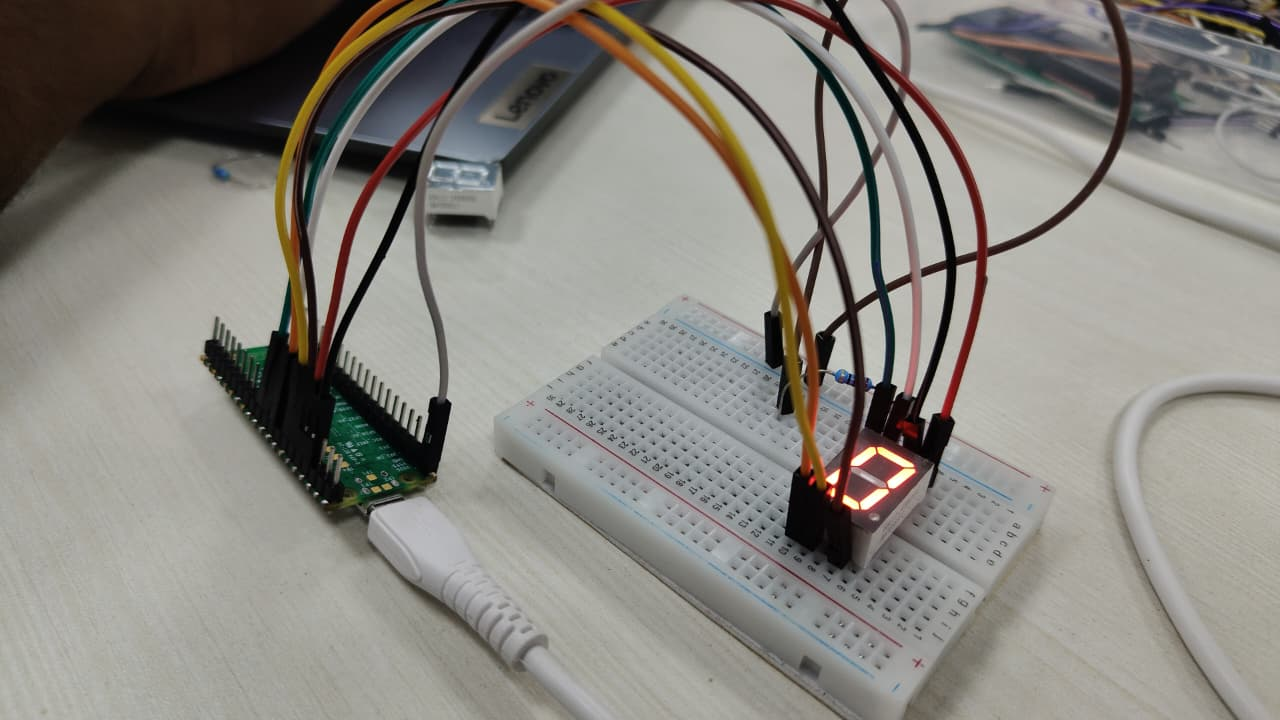
\includegraphics[width=8cm]{output.jpeg}
\end{center}

%================ CONCLUSION ==================
\section*{Conclusion}

The given Boolean expression simplifies to:

\[
F = \overline{ABC}
\]

This represents a 3-input NAND gate.

The experimental results match the theoretical truth table.

\end{document}
